\documentclass[a4paper,12pt]{article}
\usepackage{amsmath}
\usepackage{graphicx}
\usepackage{listings}
\usepackage[table,xcdraw]{xcolor}
\usepackage{graphicx}
% Define custom settings for code listing
\lstset{
    basicstyle=\ttfamily\footnotesize,
    backgroundcolor=\color{gray!10},
    keywordstyle=\color{blue},
    commentstyle=\color{green!50!black},
    stringstyle=\color{red},
    breaklines=true,
    frame=single,
    numbers=left,
    numberstyle=\tiny,
    captionpos=b,
    showspaces=false,
    showstringspaces=false
}

\title{Deep Q-Learning for Flappy Bird: Implementation and Report}
\author{Alice}
\date{\today}

\begin{document}

\maketitle

\section*{Abstract}
This report presents a Deep Q-Learning (DQN) approach to train an agent to play the Flappy Bird game. The implementation involves designing a convolutional neural network (CNN) for approximating Q-values, using a replay memory for experience replay, and applying techniques such as image preprocessing and epsilon-greedy exploration. This report provides a detailed description of the architecture, methodology, and implementation in Python.

\section{Introduction}
Deep Q-Learning combines reinforcement learning with deep neural networks to solve high-dimensional state-space problems. In this project, the Flappy Bird environment is utilized to test and demonstrate the capabilities of a DQN agent. The key components of the implementation include the agent's architecture, replay memory, and image preprocessing pipeline.

\section{Code Components}
This section describes the core components of the implementation.

\subsection{DQNAgent Class}
The \texttt{DQNAgent} class defines the agent that interacts with the environment, learns from experiences, and updates its policy. Key parameters such as \texttt{batch\_size}, \texttt{gamma}, and \texttt{epsilon} are adjustable. A snippet of the class implementation is shown below:

\begin{lstlisting}[language=Python, caption=DQNAgent Implementation]
def init_weights(l):
    if type(l) == torch.nn.Linear or type(l) == torch.nn.Conv2d:
        torch.nn.init.xavier_normal_(l.weight)
        l.bias.data.fill_(0.01)

class DQNAgent:
    def __init__(self, input_shape, num_actions, batch_size=32, gamma=0.99, eps=1, eps_min=0.01, eps_decay=0.999, replay_buffer=5000):
        self.env = gymnasium.make("FlappyBird-v0", render_mode="rgb_array", use_lidar=False)
        self.device = torch.device("cuda" if torch.cuda.is_available() else "cpu")
        self.policy_net = DQN(input_shape, num_actions).to(self.device)
        self.policy_net.apply(init_weights)
        self.target_net = DQN(input_shape, num_actions).to(self.device)
        self.target_net.load_state_dict(self.policy_net.state_dict())
        self.target_net.eval()
        self.optimizer = torch.optim.Adam(self.policy_net.parameters())
        self.memory = ReplayMemory(replay_buffer)
        self.batch_size = batch_size
        self.gamma = gamma
        self.eps = eps
        self.eps_min = eps_min
        self.eps_decay = eps_decay
\end{lstlisting}

\subsection{Replay Memory}
Replay memory is implemented using a double-ended queue (deque) to store experiences and allow random sampling for training. This improves stability and efficiency. The implementation is as follows:

\begin{lstlisting}[language=Python, caption=Replay Memory]
from collections import deque
from random import sample

class ReplayMemory:
    def __init__(self, capacity):
        self.memory = deque(maxlen=capacity)

    def push(self, state, action, reward, next_state, done):
        self.memory.append((state, action, reward, next_state, done))

    def __len__(self):
        return len(self.memory)

    def sample(self, batch_size):
        return sample(self.memory, batch_size)
\end{lstlisting}

\subsection{Deep Q-Network (DQN)}
The DQN is a convolutional neural network designed to process image inputs and predict Q-values for actions. It includes convolutional layers, fully connected layers, and dropout for regularization. The implementation is as follows:

\begin{lstlisting}[language=Python, caption=DQN Architecture]
import torch.nn as nn
import torch.nn.functional as F
import torch
import numpy as np

class DQN(nn.Module):
    def __init__(self, input_shape, num_actions):
        super(DQN, self).__init__()
        self.conv1 = nn.Conv2d(in_channels=input_shape[0], out_channels=4, kernel_size=8, stride=4)
        self.conv2 = nn.Conv2d(in_channels=4, out_channels=8, kernel_size=4, stride=2)
        self.fc1 = nn.Linear(self._compute_conv_out(input_shape), 64)
        self.fc2 = nn.Linear(64, num_actions)
        self.dropout = nn.Dropout(p=0.2)

    def _compute_conv_out(self, shape):
        x = torch.zeros(1, *shape)
        x = self.conv1(x)
        x = self.conv2(x)
        return int(np.prod(x.size()))

    def forward(self, x):
        x = F.relu(self.conv1(x))
        x = F.relu(self.conv2(x))
        x = x.view(x.size(0), -1)
        x = F.relu(self.fc1(x))
        x = self.dropout(x)
        x = self.fc2(x)
        return x
\end{lstlisting}

\subsection{Image Preprocessing}
To improve the agent's performance, image frames are preprocessed by resizing, applying color masks, and generating binary states. The \texttt{process\_image} function is implemented as follows:

\begin{lstlisting}[language=Python, caption=Image Preprocessing]
def process_image(image):
    image = image[20:380, :, :]
    image = cv2.resize(image, (72, 72))

    bird_1 = image[:, :, 0]
    bird_1[bird_1 > 227] = 255
    bird_1[bird_1 <= 227] = 0

    bird_2 = image[:, :, 2]
    bird_2[bird_2 > 138] = 255
    bird_2[bird_2 <= 138] = 0

    bird = np.zeros((72, 72))
    bird[(bird_1 == 255) | (bird_2 == 255)] = 255

    pipes = image[:, :, 1]
    pipes[pipes > 136] = 255
    pipes[pipes <= 136] = 0

    final_state = np.where(pipes == 255, 1, 0)
    final_state = np.where(bird == 255, 0.5, final_state)
    return final_state
\end{lstlisting}

\subsection{Testing Player}
This agent would take a model that was pretrained by our implementations and uses it to play Flappy Birds. It tries to play 5 games and outputs the final rewards received,
whilst showcasing the gameplay itself. It's implementation is shown below:
\begin{lstlisting}[language=Python, caption=Testing player]
import torch
import gymnasium
import flappy_bird_gymnasium
from utils.dqn import DQN
from utils.img_processor import process_image
import numpy as np

class DQNPlayer:
    def __init__(self, model_path, input_shape, num_actions, seed=42):
        self.env_rgb = gymnasium.make("FlappyBird-v0", render_mode="rgb_array",use_lidar = False)
        self.env_human = gymnasium.make("FlappyBird-v0", render_mode="human",use_lidar = False)
        self.device = torch.device("cuda" if torch.cuda.is_available() else "cpu")

        self.env_rgb.reset(seed=seed)
        self.env_human.reset(seed=seed)

        self.policy_net = DQN(input_shape, num_actions).to(self.device)
        self.policy_net.load_state_dict(torch.load(model_path, map_location=self.device))
        self.policy_net.eval()  

    def play(self, episodes=5):
        for episode in range(episodes):
            seed = np.random.randint(0, 10000)  
            state_rgb, _ = self.env_rgb.reset(seed=seed)
            self.env_human.reset(seed=seed)  

            frame = self.env_rgb.render()  
            if frame is None:
                raise ValueError("Rendered frame is None. Check environment's render_mode.")
            state = process_image(frame)
            state = np.stack([state] * 4, axis=0)  

            done = False
            total_reward = 0

            while not done:
                self.env_human.render()

                state_tensor = torch.FloatTensor(state).unsqueeze(0).to(self.device)
                with torch.no_grad():
                    action = self.policy_net(state_tensor).argmax(dim=1).item()

                _, reward, done, _, _ = self.env_rgb.step(action)
                self.env_human.step(action) 
                total_reward += reward
    
                    
                frame = self.env_rgb.render()
                if frame is None:
                    raise ValueError("Rendered frame is None during gameplay.")
                next_state = process_image(frame)
                state = np.append(state[1:], [next_state], axis=0)  
            print(f"Episode {episode + 1}: Total Reward = {total_reward:.1f}")

        self.env_rgb.close()
        self.env_human.close()

if __name__ == "__main__":
    model_path = "models/best_model_62.6.pth" 
    player = DQNPlayer(model_path, input_shape=(4, 72, 72), num_actions=2, seed=42)
    player.play(episodes=5)
\end{lstlisting}


\section{Training}
The training loop runs for a specified number of epochs. During each episode, the agent interacts with the environment, collects experiences, and updates the policy network using the Bellman equation. Target networks are periodically updated to stabilize learning.

\subsection{Hyperparameters and Results}
The performance of the DQN agent depends significantly on the choice of hyperparameters. The following table summarizes the hyperparameters used in this implementation:
We tested two sets of hyperparameters , modifying the replay buffer and the number of epochs after witch the model trains on mini-batches.
\begin{table}[ht!]
    \centering
    \begin{tabular}{|l|c|}
        \hline
        \textbf{Hyperparameter} & \textbf{Value} \\
        \hline
        Batch Size & 32 \\
        \rowcolor{lime}
        Replay Memory Capacity & 50,000 \\
        Discount Factor ($\gamma$) & 0.95 \\
        Initial Epsilon ($\epsilon$) & 1.0 \\
        Minimum Epsilon ($\epsilon_{min}$) & 0.01 \\
        Epsilon Decay Rate & 0.999 \\
        Learning Rate & 0.001 \\
        \rowcolor{lime}
        Target Network Update Frequency & 5 epochs \\
        Training Episodes & 10,000 \\
        Input Image Dimensions & (72, 72) \\
        \hline
    \end{tabular}
    \caption{Second set of hyperparameters used in training the DQN agent.}
    \label{tab:hyperparameters}
\end{table}

\begin{figure}[ht!]
    \centering
    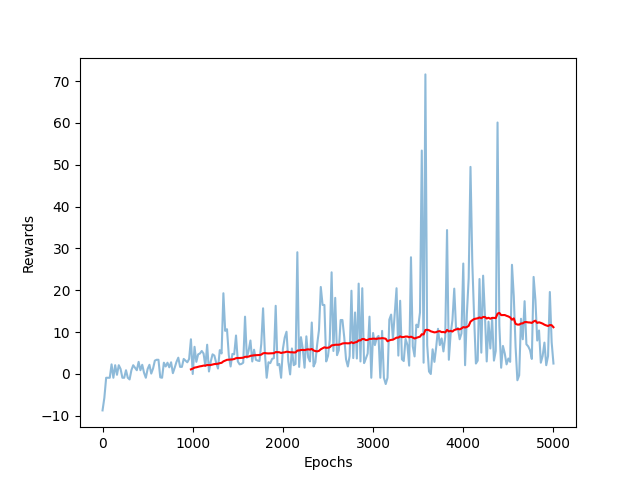
\includegraphics[width=0.8\textwidth]{first_run.png} 
    \caption{Learning curve: Cumulative return achieved per episode during training using the second set of hyperparameters.}
    \label{fig:learning_curve}
\end{figure}

\begin{table}[ht!]
    \centering
    \begin{tabular}{|l|c|}
        \hline
        \textbf{Hyperparameter} & \textbf{Value} \\
        \hline
        Batch Size & 32 \\
        \rowcolor{lime}
        Replay Memory Capacity & 25,000 \\
        Discount Factor ($\gamma$) & 0.95 \\
        Initial Epsilon ($\epsilon$) & 1.0 \\
        Minimum Epsilon ($\epsilon_{min}$) & 0.01 \\
        Epsilon Decay Rate & 0.999 \\
        Learning Rate & 0.001 \\
        \rowcolor{lime}
        Target Network Update Frequency & 10 epochs \\
        Training Episodes & 10,000 \\
        Input Image Dimensions & (72, 72) \\
        \hline
    \end{tabular}
    \caption{First set of hyperparameters used in training the DQN agent.}
    \label{tab:hyperparameters2}
\end{table}

\begin{figure}[ht!]
    \centering
    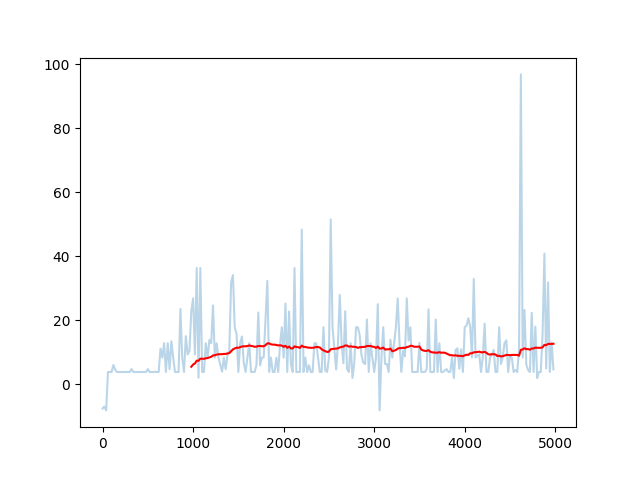
\includegraphics[width=0.8\textwidth]{second_plot.png} 
    \caption{Learning curve: Cumulative return achieved per episode during training using the first set of hyperparameters.}
    \label{fig:learning_curve2}
\end{figure}
As we can see from the results, using a larger replay buffer tends to lead to a more stable learning curve, yet the Neural Network learns at a
slower pace. Meanwhile, using a smaller value for the replay buffer, the network starts learning somewhat faster, but reaches a pleatou much quicker
and doesn't show that much improvement. 
\\ \\
\section{Other solutions}
At first, we tried implementing a Actor Critic model for the Neural Network, but we saw some problems that we found hard to fix with that approach.
Mainly, we saw the model tending to prioritize getting quick, easy and guaranteed rewards in the short term, rather than taking risks in order to achieve some long term, higher
rewards. Because of that , the scores received in training reached pleatous really quickly and were not very high, meaning the model was pretty weak at completing it's task.
This was the reason why we switched to DQN, where a single neural network is doing the job of both the Actor and the Critic, and it shows massive improvements.
\section{Conclusion}
This project demonstrates the application of Deep Q-Learning to a challenging environment like Flappy Bird. The implementation highlights key aspects such as efficient memory management, CNN-based Q-function approximation, and effective image preprocessing. Future work could involve experimenting with hyperparameters and exploring alternative architectures.

\end{document}
